\documentclass[11pt, a4paper]{article}
% Set the fonts of the document
\usepackage{inconsolata} % Monospace font
\usepackage{helvet} % Sans-serif font
\usepackage[
    libertine, % do not override the sans-serif-font
    tt = false % do not override the monospace font
]{libertine} % Main font (serif)

\usepackage[
    top = 3cm,
    bottom = 3cm,
    left = 2.5cm,
    right = 2.5cm
]{geometry}

\usepackage[english]{babel}
\usepackage{xspace}
\usepackage{booktabs}
\usepackage{enumitem}
\usepackage[xcolor]{mdframed}
\usepackage{amsmath}
\usepackage{amssymb}
\usepackage{amsthm}
\usepackage{mathrsfs}
\usepackage{stmaryrd}
\usepackage{float}
\usepackage{listings}
\usepackage{parskip}
\usepackage[
    labelfont = {small, bf},
    textfont = {small}
]{caption}
\usepackage{subcaption}
\usepackage{circledsteps}
\usepackage{hyperref}

% ====================================================================

\newcommand{\eg}{e.g.,\xspace}
\newcommand{\ie}{i.e.\xspace}
\newcommand{\etal}{\textit{et~al.}\xspace}

\newcommand{\todo}[1]{{\centering\textbf{\textcolor{red}{[TODO : #1]}}\xspace}}

\newcommand{\vsc}{Visual Studio Code\xspace}

\DeclareRobustCommand{\iLaTeX}{\mbox{{{\itshape i}-\hspace{-0.25mm}}\LaTeX{}}}

% Document title
\newcommand{\makedoctitle}[1]{%
\begin{center}
    \color{black!75}
    {\Large{Longitudinal study of \iLaTeX}} \\
    \noindent\rule{12cm}{0.4pt} \\[1.5em]
    \color{black}
    {\Huge{#1}} \\[0.5em]
    % \noindent\rule{16cm}{0.4pt}
\end{center}
}

% Custom framed environments
\newmdenv[
    linecolor = red!50!black,
    backgroundcolor = red!2,
    skipabove = 1em,
    skipbelow = 1em,
    innertopmargin = 1em,
    innerbottommargin = 1em,
    frametitle = {Warning},
    frametitlebackgroundcolor = red!5,
    % startinnercode = \centering\bgroup,
    % endinnercode = \egroup
    nobreak = true
]{warning}

\newmdenv[
    linecolor = blue!50!black,
    backgroundcolor = blue!2,
    skipabove = 1em,
    skipbelow = 1em,
    innertopmargin = 1em,
    innerbottommargin = 1em,
    frametitle = {Good to know},
    frametitlebackgroundcolor = blue!5,
    % startinnercode = \centering\bgroup,
    % endinnercode = \egroup
    nobreak = true
]{info}

\newmdenv[
    linecolor = green!50!black,
    backgroundcolor = green!2,
    skipabove = 1em,
    skipbelow = 1em,
    innertopmargin = 1em,
    innerbottommargin = 1em,
    frametitle = {Example},
    frametitlebackgroundcolor = green!5,
    % startinnercode = \centering\bgroup,
    % endinnercode = \egroup,
    % nobreak = true
]{example}

% Style of code blocks
\lstdefinestyle{custom-latex}{
    language={[LaTeX]TeX},
    backgroundcolor=\color{white},
    commentstyle=\color{black!50},
    keywordstyle=\color{green!50!black},
    numberstyle=\tiny\color{red!50!black},
    stringstyle=\color{blue!50!black},
    basicstyle=\ttfamily\small,
    breakatwhitespace=false,         
    breaklines=true,
    keepspaces=true,
    numbers=none,
    tabsize=4,
    aboveskip={1em},
    belowskip={0.7em}
}

\lstdefinestyle{custom-latex-example}{
    language={[LaTeX]TeX},
    commentstyle=\color{black!50},
    keywordstyle=\color{green!50!black},
    numberstyle=\tiny\color{red!50!black},
    stringstyle=\color{blue!50!black},
    basicstyle=\ttfamily\footnotesize,
    breakatwhitespace=false,         
    breaklines=true,
    keepspaces=true,
    numbers=none,
    tabsize=4,
    aboveskip={1em},
    belowskip={-1ex}
}

% Description of a command/environment (for the cheat sheet)
\newcommand{\commanddesc}[1]{{\color{black!80}{#1}}}


% Command to produce a circled number to reference a step represented in a figure
\definecolor{FigStepColor}{HTML}{BC43F0}

\DeclareRobustCommand{\figstep}[1]{%
    \Circled[%
        inner color=white,%
        outer color=white,%
        fill color=FigStepColor%
    ]{\sffamily\textbf{#1}}%
}

% This package is required for iLaTeX to work!
\usepackage{ilatex}

\begin{document}

\makedoctitle{Introduction to \iLaTeX{}}

%%%%%%%%%%%%%%%%%%%%%%%%%%%%%%%% START OF CONTENT

\section{What is \iLaTeX{}?}
\iLaTeX{} is a research prototype of a new kind of editor for \LaTeX{} documents.
It is built on top of Visual Studio Code, an open-source code editor.
\iLaTeX{} looks and works like other \LaTeX{} editors such as TeXstudio and Overleaf, but it also offers a new kind of features we call \emph{interactive intermediate representations}---or IIR for short.

IIRs constitute an alternative way to visualise and manipulate certain parts of a \LaTeX{} document than the source code or the generated PDF.
Each IIR is bound to a piece of \emph{visualisable code}, \ie code that can be visualised through an IIR.
IIR are an optional feature of \iLaTeX{}: since the source code of your documents remains accessible at all times, you can also use \iLaTeX{} like a standard \LaTeX{} editor!



\section{\iLaTeX{} in this study}

This study is made of two successive parts that are independent from each other.
At some points in the study, you may be requested or forbidden to use IIRs by the investigator:
\begin{itemize}
    \item If you are \textbf{requested} to use IIRs, you should use IIR as much as possible to perform the task you have been assigned. However, if you believe you cannot accomplish what you want to do with an IIR, or if you think editing the code directly would be faster, you are still allowed to use the code editor.
    \item If you are \textbf{forbidden} to use IIRs, you must use \iLaTeX{} like a standard code editor (you can still use all the regular code editing features provided by Visual Studio Code such as search-and-replace and keyboard shortcuts);
    \item \textbf{Otherwise}, you are free to decide whether you want to use IIRs or not!
\end{itemize}

In case of doubt of whether you can or should use IIR for the current task, please ask the investigator.



\section{General usage of \iLaTeX{}}
\iLaTeX{} will automatically attempt to find all pieces of visualisable code in your document and to create an IIR for every of them.
Visualisable code is detected by the usage of \textbf{special \LaTeX{} commands and environments} that are known to be visualisable by \iLaTeX{}. They will be explained in more details in the next section.

Most of the time, the IIR associated to a PDF element with a \textbf{blue halo} can be displayed by clicking on it.
In some situations however, an IIR may be \textbf{disabled}. In this case, you may encounter the following visuals:

\newpage
\begin{minipage}[t][2.5cm][c]{0.45\textwidth}
    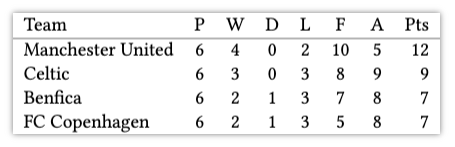
\includegraphics[width=\textwidth]{img/disabled-table.png}
\end{minipage}
\hspace{0.05\textwidth}
\begin{minipage}[t][2.5cm][c]{0.5\textwidth}
    A \textbf{grey halo} means the IIR is disabled: it cannot be clicked.
    It happens (1) every time the document is \textbf{compiling} or (2) when the \textbf{compilation fails}.
\end{minipage}
\begin{minipage}[t][2.5cm][c]{0.45\textwidth}
    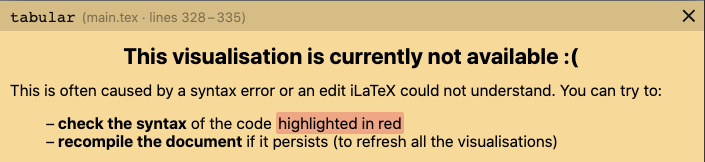
\includegraphics[width=\textwidth]{img/syntax-error-in-visualisation.png}
\end{minipage}
\hspace{0.05\textwidth}
\begin{minipage}[t][2.5cm][c]{0.5\textwidth}
    If you edit visualisable code \textbf{while its IIR is displayed}, \iLaTeX{} may (1) fail at \textbf{parsing your code} or (2) \textbf{loose track} of the code.
    In this case, either fix the syntax or recompile \mbox{the document} to force \iLaTeX{} to re-detect every piece of \mbox{visualisable code}.
\end{minipage}



%%%%%%%%%%%%%%%%%%%%%%%%%%%%%%%%

\newpage
\section{List of IIRs available in \iLaTeX{}}

% \newpage
\subsection{Mathematics}

\begin{figure}[hb!]
    \centering
    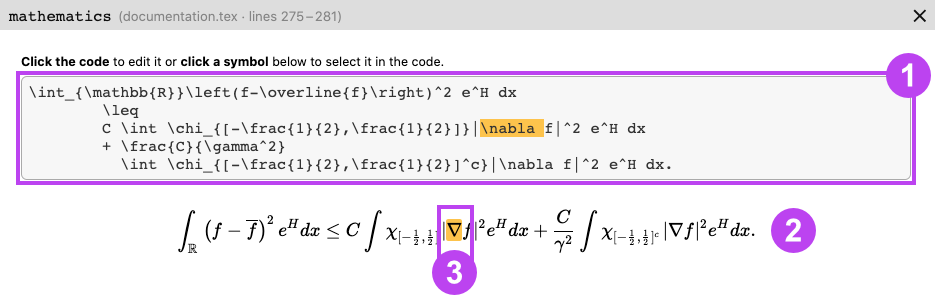
\includegraphics[width = \textwidth]{img/iir-imaths.png}
    \caption{The IIR of \texttt{imaths} environments. \figstep{1} The editable code of the formula. You can click it to \textbf{modify the code}, and the typeset formula will be \textbf{updated in real time}. \figstep{2} A typeset formula representing the code displayed above. \figstep{3} You can \textbf{point} and \textbf{click} most symbols in the typeset formula to respectively \textbf{highlight} or \textbf{select the piece of code} that generated it.}
    \label{fig:iir-imaths}
\end{figure}

An IIR for mathematics (\autoref{fig:iir-imaths}) can be created with the \texttt{imaths} environment:

\begin{lstlisting}[style=custom-latex]
\begin{imaths}
    x = \alpha x + \beta y + \gamma
\end{imaths}
\end{lstlisting}

It behaves like the \texttt{align*} environment provided by the \texttt{amsmath} package: you can use all the commands accepted by \LaTeX{} in math mode inside, and you can align several formulae by using \verb|&| to align symbols vertically and \verb|\\| to break lines.

% This IIR enables you to edit the code of the formula and \textbf{see the change in the typeset formula in real time}, as well as to \textbf{find} (by pointing) and to \textbf{select} (by clicking) the piece of code related to almost every symbol of the typeset formula.

% \begin{info}
%     When you edit the code of the formula in the IIR, the actual code of your \LaTeX{} document will \textbf{not} be updated until you click outside of the text area or press Enter.
% \end{info}

\begin{warning}
    User-defined commands are not supported (it will compile, but the IIR will not work correctly).
\end{warning}

\begin{example}
    Try to click the formula below and to edit it using the IIR.
    
    \begin{imaths}
        \int_{\mathbb{R}}\left(f-\overline{f}\right)^2 e^H dx \leq C \int \chi_{[-\frac{1}{2},\frac{1}{2}]}|\nabla f|^2 e^H dx +\frac{C}{\gamma^2}  \int \chi_{[-\frac{1}{2},\frac{1}{2}]^c}|\nabla f|^2 e^H dx.
    \end{imaths}
\end{example}


%%%%%%%%%%%%%%%%%%%%%%%%%%%%%%%%


\newpage
\subsection{Images}

\begin{figure}[h!]
    \centering
    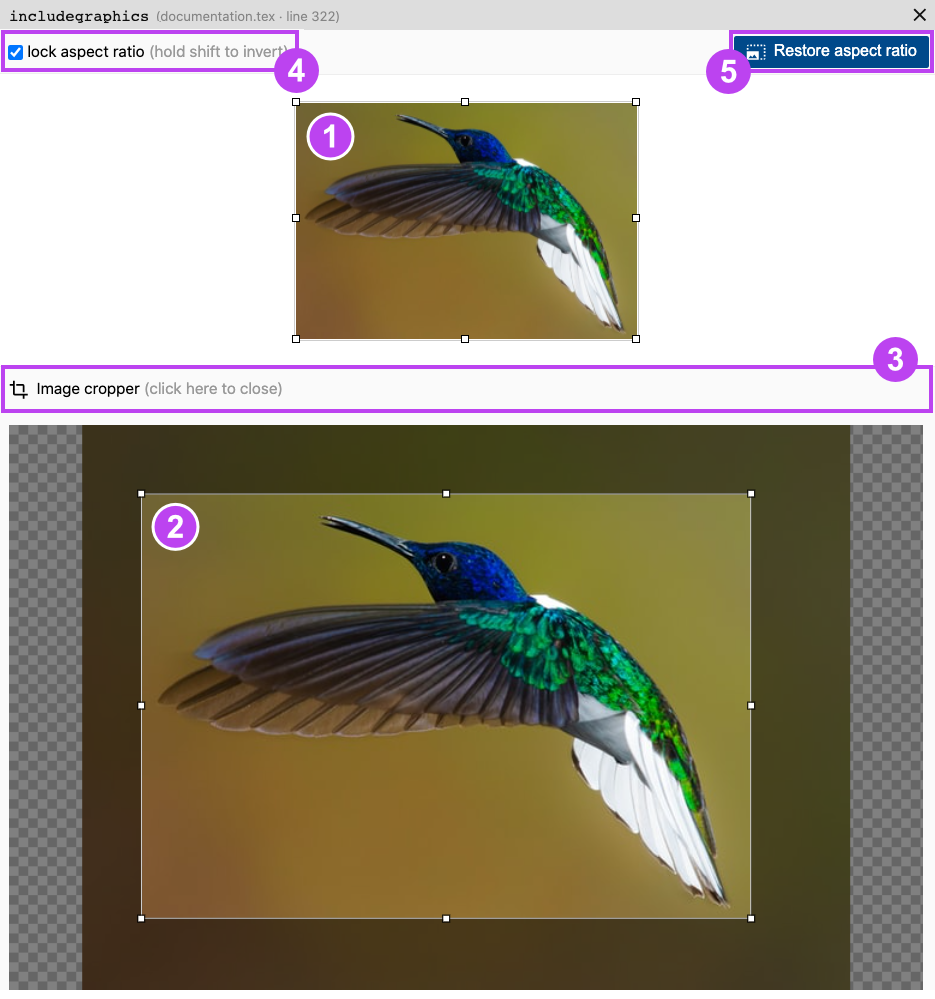
\includegraphics[width = .75\textwidth]{img/iir-iincludegraphics.png}
    \caption{The IIR of \texttt{iincludegraphics} commands. \figstep{1} The expected output of the command. You can \textbf{resize it} by dragging one of the handles around the image. \figstep{2} The area of the image to display. You can \textbf{move it} by dragging it and \textbf{resize it} by dragging one of the handles around the visible area. \figstep{3} You can display or hide the image cropper by clicking this bar. \figstep{4} You can hold the Shift key or uncheck this box to resize the image with a \textbf{non-natural aspect ratio}. If the image has a non-natural aspect ratio when the IIR is opened, the box will be unchecked by default. \figstep{5} You can resize the image to \textbf{restore its natural aspect ratio} by clicking this button.}
    \label{fig:iir-iincludegraphics}
\end{figure}

An IIR for images (\autoref{fig:iir-inicluegraphics}) can be created with the \verb|\iincludegraphics| command (with two \texttt{i}s!):

\begin{lstlisting}[style=custom-latex]
\iincludegraphics[width=\textwidth]{path/to/your/image.png}
\end{lstlisting}

It behaves like the \verb|\includegraphics| command provided by the \texttt{graphicx} package.
Only the \texttt{width}, \texttt{height}, \texttt{trim} and \texttt{clip} options are recognised by \iLaTeX{}.
You can still use all the other options supported by \verb|\includegraphics|, but the IIR will ignore them and may delete them.

% This IIR enables you to \textbf{resize} and to \textbf{crop} the image (\ie only display a certain region of the image). To resize the image (top widget) or the cropped region (bottom widget), click and drag one of the handles displayed around the frame.

\begin{info}
    \iLaTeX{} supports the most common \emph{length macros} like \verb|\textwidth|, so you can freely use them in the options.
    If you are unsure whether a less common length macro is supported and want to use it, please ask the investigator.
\end{info}

% \begin{warning}
%     PDF images are not supported (it will compile, but the IIR will not work correctly).
% \end{warning}

\begin{example}
    Try to click the image below and to edit it using the IIR.
    
    \centering
    \iincludegraphics[width = 0.5\textwidth]{img/bird.jpg}
\end{example}


%%%%%%%%%%%%%%%%%%%%%%%%%%%%%%%%


\newpage
\subsection{Tables}

\begin{figure}[hb!]
    \centering
    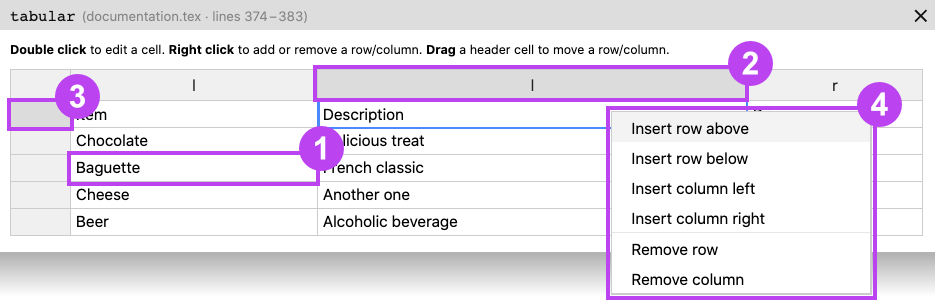
\includegraphics[width = \textwidth]{img/iir-itabular.png}
    \caption{The IIR of \texttt{itabular} environments. \figstep{1} A cell of the table. You can \textbf{edit} its content by double-clicking on it. \figstep{2} The header cell of a column. If \iLaTeX{} was able to parse the type of this column (\eg \texttt{l}, \texttt{c}, \texttt{r}), this cell contains it. You can \textbf{drag it} to \textbf{move the column}. \figstep{3} The header cell of a row. You can \textbf{drag it} to \textbf{move the row}. \figstep{4} You can display a \textbf{contextual menu} by right-clicking any cell of the table. It enables you to \textbf{insert} and \textbf{delete} \textbf{rows and columns}.}
    \label{fig:iir-itabular}
\end{figure}

An IIR for tables (\autoref{fig:iir-itabular}) can be created with the \texttt{itabular} environment:

\begin{lstlisting}[style=custom-latex]
\begin{itabular}{llr}
    Item      & Description & Price \\
    Chocolate & ...         & 2.20  \\
    Baguette  & ...         & 0.90
\end{itabular}
\end{lstlisting}

It behaves like the \texttt{tabular} environment, and expects one mandatory argument (the specification of the columns, such as \texttt{l}, \texttt{r}, etc).

% This IIR enables you to \textbf{edit any cell} (by double-clicking it), to \textbf{insert and delete} rows and columns (via a contextual menu displayed on right click), and to \textbf{move} rows and columns (by dragging and dropping the header cell of the row/column).

% \begin{info}
%     Common formatting commands for tables such as \verb|\hline|, \verb|\toprule|, \verb|\midrule| and \verb|\bottomrule| are not considered as ``cell content'' by this IIR. You can safely use them, and \iLaTeX{} will do its best to ignore them and leave them in place.
% \end{info}

% \begin{warning}
%     Merged cells are not supported (it will compile, but the IIR will not work correctly).
% \end{warning}

\begin{example}
    Try to click the table below and to edit it using the IIR.
    
    \centering
    \begin{itabular}{llr}
        \toprule
        Item  & Description & Price \\
        \midrule
        Chocolate & Delicious treat & 2.20  \\
        Baguette & French classic & 0.90  \\
        Cheese & Another one & 3.00  \\
        Beer & Alcoholic beverage & 4.50  \\
        \bottomrule
    \end{itabular}
\end{example}


%%%%%%%%%%%%%%%%%%%%%%%%%%%%%%%%


\newpage
\section{Summary of every special commands and environments}
Do not forget to adapt the parameters as needed!

\subsection*{Mathematics}

\commanddesc{Insert a single- or multi-line formula}
\hfill
\lstinline[style=custom-latex]|\begin{imaths} f(x) = 1 \end{imaths}|



\subsection*{Images}

\commanddesc{Insert an image}
\hfill
\lstinline[style=custom-latex]|\iincludegraphics[width=\textwidth]{image.png}|



\subsection*{Tables}

\commanddesc{Insert tabulated data}
\hfill
\lstinline[style=custom-latex]|\begin{itabular}{ll} a & b \\ c & d \end{itabular}|


%%%%%%%%%%%%%%%%%%%%%%%%%%%%%%%% END OF CONTENT

\end{document}
